\documentclass[aspectratio=169]{beamer}
\usepackage[utf8]{inputenc}
\usepackage{graphicx}
\usepackage{amsmath}
\usepackage{amssymb}
\usepackage{xcolor}
\usepackage{tikz}
\usepackage{pifont}
\usepackage{colortbl}
\usepackage{booktabs}
\usepackage{tabularx}
\usetikzlibrary{arrows.meta,shadows,shapes.geometric,positioning,fit,backgrounds,calc}

\IfFileExists{fontawesome5.sty}{
  \usepackage{fontawesome5}
  \newcommand{\icoThumb}{\faThumbsUp}
  \newcommand{\icoWarn}{\faExclamationTriangle}
  \newcommand{\icoIdea}{\faLightbulb}
  \newcommand{\icoCogs}{\faCogs}
  \newcommand{\icoBrain}{\faBrain}
  \newcommand{\icoDB}{\faDatabase}
  \newcommand{\icoPy}{\faPython}
  \newcommand{\icoServer}{\faServer}
  \newcommand{\icoDocker}{\faDocker}
  \newcommand{\icoNet}{\faNetworkWired}
  \newcommand{\icoRocket}{\faRocket}
  \newcommand{\icoCode}{\faCode}
  \newcommand{\icoLink}{\faLink}
  \newcommand{\icoBan}{\faBan}
  \newcommand{\icoRoad}{\faRoad}
  \newcommand{\icoStar}{\faStar}
  \newcommand{\icoChart}{\faChartBar}
  \newcommand{\icoCheck}{\faCheckCircle}
  \newcommand{\icoX}{\faTimesCircle}
  \newcommand{\icoUser}{\faUser}
  \newcommand{\icoCloud}{\faCloud}
  \newcommand{\icoGrad}{\faGraduationCap}
  \newcommand{\icoUni}{\faUniversity}
  \newcommand{\icoCal}{\faCalendar} % Corretto da \faCalendarAlt a \faCalendar
  \newcommand{\icoTeach}{\faChalkboardTeacher}
  \newcommand{\icoKey}{\faKey}
  \newcommand{\icoPlay}{\faPlay}
  \newcommand{\icoAnsible}{\faTools}
}{
  \usepackage{pifont}
  \newcommand{\icoThumb}{\textbf{+}}
  \newcommand{\icoWarn}{\textbf{!}}
  \newcommand{\icoIdea}{\textbf{$\bigstar$}}
  \newcommand{\icoCogs}{\ding{102}}
  \newcommand{\icoBrain}{\ding{108}}
  \newcommand{\icoDB}{\ding{110}}
  \newcommand{\icoPy}{\ding{228}}
  \newcommand{\icoServer}{\ding{111}}
  \newcommand{\icoDocker}{\ding{117}}
  \newcommand{\icoNet}{\ding{213}}
  \newcommand{\icoRocket}{\ding{224}}
  \newcommand{\icoCode}{\texttt{</>}}
  \newcommand{\icoLink}{\ding{212}}
  \newcommand{\icoBan}{\ding{55}}
  \newcommand{\icoRoad}{\ding{229}}
  \newcommand{\icoStar}{\ding{72}}
  \newcommand{\icoChart}{\ding{115}}
  \newcommand{\icoCheck}{\ding{52}}
  \newcommand{\icoX}{\ding{56}}
  \newcommand{\icoUser}{\ding{110}}
  \newcommand{\icoCloud}{\ding{117}}
  \newcommand{\icoGrad}{\ding{72}}
  \newcommand{\icoUni}{\ding{110}}
  \newcommand{\icoCal}{\ding{111}}
  \newcommand{\icoTeach}{\ding{228}}
  \newcommand{\icoKey}{\ding{45}}
  \newcommand{\icoPlay}{\ding{228}}
  \newcommand{\icoAnsible}{\ding{46}}
}

\usetheme{metropolis}
\usecolortheme{default}

\definecolor{primaryDark}{RGB}{45,55,72}
\definecolor{accentBlue}{RGB}{66,153,225}
\definecolor{darkGray}{RGB}{74,85,104}
\definecolor{lightGray}{RGB}{247,250,252}
\definecolor{mediumGray}{RGB}{160,174,192}
\definecolor{successGreen}{RGB}{72,187,120}
\definecolor{warningRed}{RGB}{245,101,101}
\definecolor{graphsageBlue}{RGB}{41,128,185}
\definecolor{transeGreen}{RGB}{39,174,96}
\definecolor{hashgnnPurple}{RGB}{142,68,173}
\definecolor{unigold}{RGB}{204,153,0}

\setbeamercolor{palette primary}{bg=primaryDark,fg=white}
\setbeamercolor{palette secondary}{bg=accentBlue,fg=white}
\setbeamercolor{palette tertiary}{bg=darkGray,fg=white}
\setbeamercolor{frametitle}{bg=primaryDark,fg=white}
\setbeamercolor{block title}{bg=primaryDark,fg=white}
\setbeamercolor{block body}{bg=lightGray,fg=darkGray}
\setbeamercolor{alerted text}{fg=warningRed}
\setbeamercolor{example text}{fg=successGreen}
\setbeamercolor{normal text}{fg=darkGray,bg=white}
\setbeamercolor{structure}{fg=primaryDark}
\setbeamercolor{progress bar}{fg=accentBlue,bg=mediumGray!40}

\setbeamertemplate{frame numbering}[fraction]
\setbeamertemplate{footline}{
  \leavevmode
  \hbox{%
    \begin{beamercolorbox}[wd=.5\paperwidth,ht=2.5ex,dp=1ex,left,leftskip=1em]{author in head/foot}%
      \usebeamerfont{author in head/foot}\textbf{Sandi Russo} \hspace{0.3cm}|\hspace{0.3cm}\textit{UniME -- Scienze Informatiche}
    \end{beamercolorbox}%
    \begin{beamercolorbox}[wd=.5\paperwidth,ht=2.5ex,dp=1ex,right,rightskip=1em]{date in head/foot}%
      \usebeamerfont{date in head/foot}\insertframenumber{} / \inserttotalframenumber
    \end{beamercolorbox}}
  \vskip0pt
}
\setbeamertemplate{navigation symbols}{}

\tikzset{
  modernbox/.style={
    rectangle, rounded corners=3pt, draw=primaryDark, thick,
    fill=lightGray, drop shadow={shadow xshift=1.5pt,shadow yshift=-1.5pt,opacity=0.25}
  },
  technode/.style={
    circle, draw=primaryDark, thick, minimum size=1.1cm,
    drop shadow={shadow xshift=1pt,shadow yshift=-1pt,opacity=0.3}
  },
  modernArrow/.style={->, thick, >=stealth, color=primaryDark}
}

\newcommand{\pro}{{\color{successGreen}\icoCheck}}
\newcommand{\con}{{\color{warningRed}\icoX}}
\newcommand{\neu}{{\color{unigold}$\sim$}}

\title[GraphSAGE vs TransE vs HashGNN]{Graph Embeddings su PharMeBiNet}
% Uso \texorpdfstring per evitare i warning di hyperref sui simboli matematici nei metadati PDF
\subtitle{Analisi Comparativa: GraphSAGE \texorpdfstring{$\cdot$}{ } TransE \texorpdfstring{$\cdot$}{ } HashGNN}
\author{Sandi Russo}
\institute{Universit\`a degli Studi di Messina\\Corso di Laurea in Scienze Informatiche}
\date{}

\begin{document}

{
\setbeamertemplate{footline}{}
\begin{frame}
  \vspace{0.7cm}
  \begin{center}
    {\Large\textbf{Graph Embeddings su PharMeBiNet}}
    \vspace{0.3cm}
    {\large Analisi Comparativa: GraphSAGE $\cdot$ TransE $\cdot$ HashGNN}
    \vspace{0.7cm}

    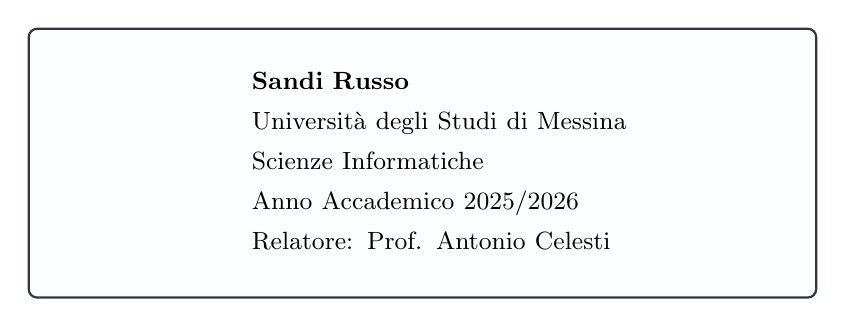
\begin{tikzpicture}
      \node[draw=primaryDark, thick, rounded corners=3pt,
            fill=lightGray!40, text width=9cm,
            align=center, inner sep=0.5cm] {
        \small
        \begin{tabular}{cl}
          \icoUser & \textbf{Sandi Russo} \\[0.12cm]
          \icoUni & Universit\`a degli Studi di Messina \\[0.12cm]
          \icoGrad & Scienze Informatiche \\[0.12cm]
          \icoCal & Anno Accademico 2025/2026 \\[0.12cm]
          \icoTeach & Relatore: Prof. Antonio Celesti \\
        \end{tabular}
      };
    \end{tikzpicture}
  \end{center}
\end{frame}
}

\begin{frame}{Agenda}
  \tableofcontents
\end{frame}

\section{Contesto e Dataset}

\begin{frame}{Contesto del Progetto}
  \centering
  \vspace{0.2cm}
  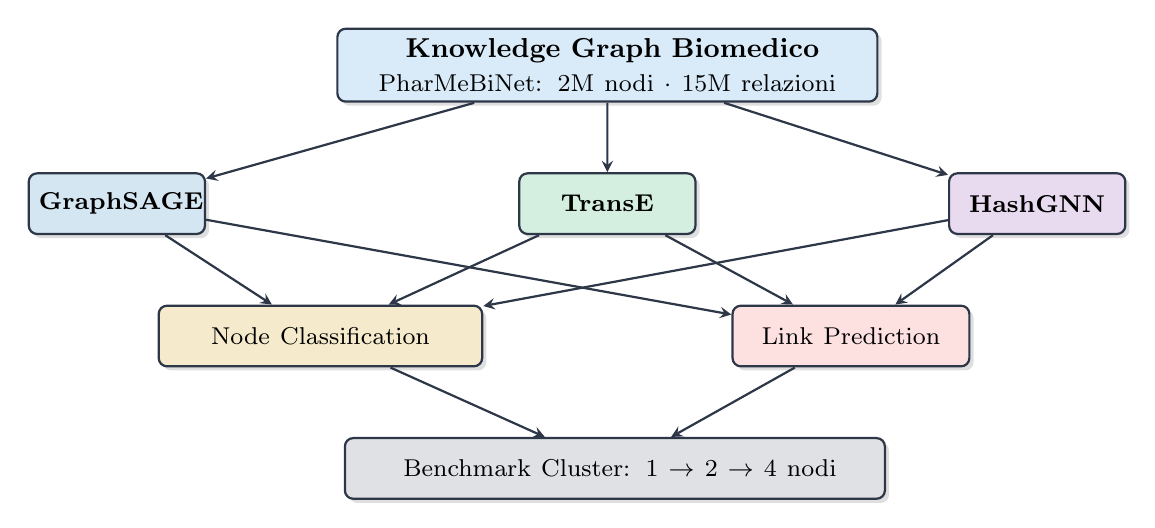
\begin{tikzpicture}[scale=1.1, transform shape, node distance=0.8cm]
    \node[modernbox, fill=accentBlue!20, text width=6cm,
          align=center, minimum height=0.8cm] (kg)
      {\small\textbf{\icoDB\ Knowledge Graph Biomedico}\\[-1pt]
       {\footnotesize PharMeBiNet: 2M nodi $\cdot$ 15M relazioni}};
    \node[modernbox, fill=graphsageBlue!20, text width=1.8cm,
          align=center, minimum height=0.7cm, below left=0.8cm and 1.5cm of kg] (gs)
      {\footnotesize\textbf{GraphSAGE}};
    \node[modernbox, fill=transeGreen!20, text width=1.8cm,
          align=center, minimum height=0.7cm, below=0.8cm of kg] (tr)
      {\footnotesize\textbf{TransE}};
    \node[modernbox, fill=hashgnnPurple!20, text width=1.8cm,
          align=center, minimum height=0.7cm, below right=0.8cm and 0.8cm of kg] (hg)
      {\footnotesize\textbf{HashGNN}};
    \draw[modernArrow] (kg) -- (gs);
    \draw[modernArrow] (kg) -- (tr);
    \draw[modernArrow] (kg) -- (hg);
    \node[modernbox, fill=unigold!20, text width=3.5cm, align=center,
          minimum height=0.7cm, below left=0.8cm and 0.4cm of tr] (nc)
      {\footnotesize Node Classification};
    \node[modernbox, fill=warningRed!20, text width=2.5cm, align=center,
          minimum height=0.7cm, below right=0.8cm and 0.4cm of tr] (lp)
      {\footnotesize Link Prediction};
    \draw[modernArrow] (gs) -- (nc); \draw[modernArrow] (gs) -- (lp);
    \draw[modernArrow] (tr) -- (nc); \draw[modernArrow] (tr) -- (lp);
    \draw[modernArrow] (hg) -- (nc); \draw[modernArrow] (hg) -- (lp);
    \node[modernbox, fill=primaryDark!15, text width=6cm, align=center,
          minimum height=0.7cm, below=0.8cm of nc, xshift=3.4cm] (cl)  
      {\footnotesize\icoCogs\ Benchmark Cluster: 1 $\to$ 2 $\to$ 4 nodi};
    \draw[modernArrow] (nc) -- (cl); \draw[modernArrow] (lp) -- (cl);
  \end{tikzpicture}
\end{frame}

\begin{frame}{Obiettivi e Stack Tecnologico}
  \begin{block}{\icoIdea\ Finalit\`a dell'Analisi}
    \small
    L'obiettivo di questo lavoro è valutare in modo strutturato quale algoritmo di embedding risulti più idoneo all'estrazione di conoscenza da reti eterogenee, analizzandone sia le prestazioni qualitative sia quelle computazionali al variare del numero di nodi del cluster.
  \end{block}
  \vspace{0.4cm}
  \begin{columns}[T]
    \begin{column}{0.48\textwidth}
      \begin{alertblock}{\icoWarn\ Domanda di Ricerca}
        \small
        Quale algoritmo offre il miglior equilibrio tra
        \textbf{qualit\`a}, \textbf{accuratezza} e
        \textbf{scalabilit\`a} su un KG biomedico fortemente eterogeneo?
      \end{alertblock}
    \end{column}
    \begin{column}{0.48\textwidth}
      \begin{block}{\icoCogs\ Stack Tecnologico}
        \small
        \begin{itemize}
          \item[\icoDB] Neo4j + APOC + GDS
          \item[\icoPy] Python: PyG, graphdatascience
          \item[\icoCloud] Azure Lab Services (8c, 32GB/VM)
          \item[\icoDocker] Docker Compose + Ansible
        \end{itemize}
      \end{block}
    \end{column}
  \end{columns}
\end{frame}

\begin{frame}{PharMeBiNet: Il Dataset}
  \begin{columns}[T]
    \begin{column}{0.46\textwidth}
      \begin{block}{\icoDB\ Pharmaceutical Mechanistic Biomedical Network}
        \footnotesize
        Knowledge Graph biomedico open-source che integra
        \textbf{oltre 20 database} (DrugBank, ChEMBL, UniProt, OMIM, \ldots).
      \end{block}
      \vspace{0.2cm}
      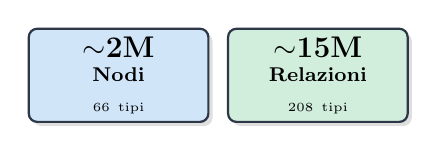
\begin{tikzpicture}[scale=0.9, transform shape]
        \node[modernbox, fill=accentBlue!25, text width=2.3cm,
              align=center, minimum height=1.1cm] (n)
          {\footnotesize\textbf{\large$\sim$2M}\\\textbf{Nodi}\\{\tiny 66 tipi}};
        \node[modernbox, fill=successGreen!25, text width=2.3cm,
              align=center, minimum height=1.1cm, right=0.25cm of n] (r)
          {\footnotesize\textbf{\large$\sim$15M}\\\textbf{Relazioni}\\{\tiny 208 tipi}};
      \end{tikzpicture}
      \vspace{0.2cm}
      \begin{alertblock}{\icoWarn\ Sfida Principale}
        \footnotesize
        L'\textbf{eterogeneit\`a} di nodi e relazioni \`e il fattore
        discriminante nella scelta dell'algoritmo.
      \end{alertblock}
    \end{column}
    \begin{column}{0.50\textwidth}
      \centering
      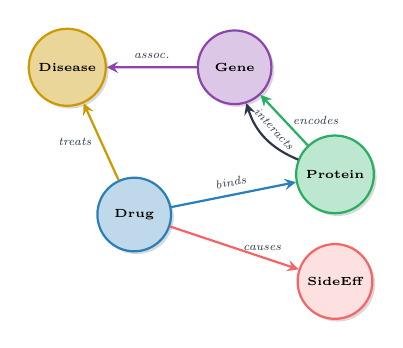
\begin{tikzpicture}[scale=0.85, transform shape,
          node/.style={technode, minimum size=1.1cm, font=\tiny\bfseries},
          rel/.style={modernArrow, font=\tiny}]
        \node[node, fill=graphsageBlue!30, draw=graphsageBlue]  (d)  at (0,0)   {Drug};
        \node[node, fill=transeGreen!30,   draw=transeGreen]    (p)  at (3,0.6) {Protein};
        \node[node, fill=hashgnnPurple!30, draw=hashgnnPurple]  (g)  at (1.5,2.2){Gene};
        \node[node, fill=unigold!40,       draw=unigold]        (di) at (-1,2.2) {Disease};
        \node[node, fill=warningRed!20,    draw=warningRed]     (se) at (3,-1)   {SideEff};
        \draw[rel, draw=graphsageBlue]  (d)  -- node[above,sloped]{\textit{binds}}    (p);
        \draw[rel, draw=unigold]        (d)  -- node[left]{\textit{treats}}           (di);
        \draw[rel, draw=transeGreen]    (p)  -- node[right]{\textit{encodes}}         (g);
        \draw[rel, draw=hashgnnPurple]  (g)  -- node[above,sloped]{\textit{assoc.}}  (di);
        \draw[rel, draw=warningRed]     (d)  -- node[right]{\textit{causes}}         (se);
        \draw[rel, draw=primaryDark]    (p)  to[bend left=25]
                                        node[above,sloped]{\textit{interacts}}        (g);
      \end{tikzpicture}
    \end{column}
  \end{columns}
\end{frame}

\section{GraphSAGE}

\begin{frame}{GraphSAGE -- Cos'\`e}
  \begin{columns}[T]
    \begin{column}{0.50\textwidth}
      \begin{block}{\icoBrain\ Definizione}
        \small
        \textbf{Graph SAmple and aggreGatE}\\
        \footnotesize Hamilton et al., 2018\\[4pt]
        Algoritmo \textbf{induttivo}: anzich\'e memorizzare un embedding
        per ogni nodo, apprende una \textbf{funzione di aggregazione}
        che generalizza anche a nodi \emph{non visti} durante il training.
      \end{block}
      \vspace{0.2cm}
      \begin{exampleblock}{\icoIdea\ Idea Chiave}
        \small
        Il vicinato di un nodo \textbf{descrive} il nodo stesso.\\
        \textit{Dimmi chi sono i tuoi vicini e ti dir\`o chi sei.}
      \end{exampleblock}
    \end{column}
    \begin{column}{0.47\textwidth}
      \centering
      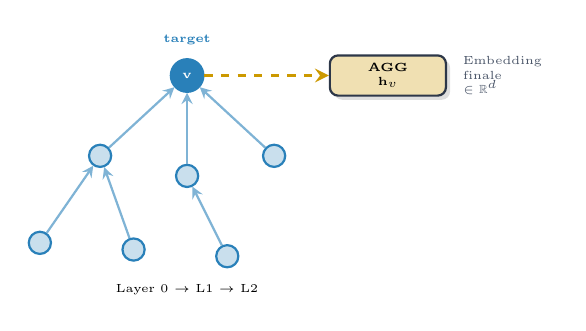
\begin{tikzpicture}[scale=0.85, transform shape,
        n/.style={circle, draw=graphsageBlue, fill=graphsageBlue!25,
                  thick, minimum size=9pt},
        nt/.style={circle, draw=graphsageBlue, fill=graphsageBlue,
                   thick, minimum size=11pt, text=white, font=\tiny\bfseries},
        arr/.style={->,thick,>=stealth,draw=graphsageBlue!60}]
        \node[nt] (v) at (0,0) {v};
        \node[n] (a) at (-1.3,-1.2) {};
        \node[n] (b) at (0,-1.5) {};
        \node[n] (c) at (1.3,-1.2) {};
        \node[n] (a1) at (-2.2,-2.5) {};
        \node[n] (a2) at (-0.8,-2.6) {};
        \node[n] (b1) at (0.6,-2.7) {};
        \draw[arr] (a)--(v); \draw[arr] (b)--(v); \draw[arr] (c)--(v);
        \draw[arr] (a1)--(a); \draw[arr] (a2)--(a); \draw[arr] (b1)--(b);
        \node[modernbox, fill=unigold!30, text width=1.5cm,
              align=center, font=\tiny\bfseries] (agg) at (3,0) {AGG\\$\mathbf{h}_v$};
        \draw[->,thick,>=stealth,draw=unigold,dashed,line width=1.2pt]
              (v) -- (agg);
        \node[font=\tiny, above=2pt of v, color=graphsageBlue]{\textbf{target}};
        \node[font=\tiny] at (0,-3.2) {Layer 0 $\to$ L1 $\to$ L2};
        \node[font=\tiny, right=0.2cm of agg, text width=1.3cm, align=left,
              color=darkGray] at (3.8,0) {Embedding\\finale\\$\in\mathbb{R}^d$};
      \end{tikzpicture}
    \end{column}
  \end{columns}
\end{frame}

\begin{frame}{GraphSAGE -- Come Funziona}
  \centering
  \vspace{0.1cm}
  % Ridotto lo scale a 0.75 per evitare l'Overfull \hbox
  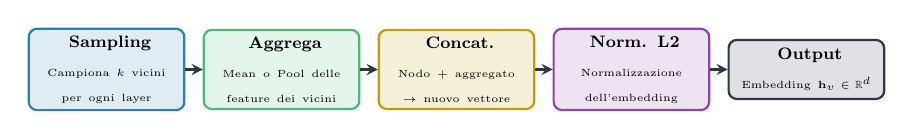
\begin{tikzpicture}[scale=0.75, transform shape, node distance=0.35cm]
    \node[rectangle,rounded corners=3pt,draw=graphsageBlue,thick,fill=graphsageBlue!15,
          text width=2.4cm,minimum height=1.0cm,text centered] (s1)
      {\footnotesize\textbf{\icoNet\ Sampling}\\[2pt]{\tiny Campiona $k$ vicini per ogni layer}};
    \node[rectangle,rounded corners=3pt,draw=successGreen,thick,fill=successGreen!15,
          text width=2.4cm,minimum height=1.0cm,text centered, right=0.3cm of s1] (s2)
      {\footnotesize\textbf{\icoBrain\ Aggrega}\\[2pt]{\tiny Mean o Pool delle feature dei vicini}};
    \node[rectangle,rounded corners=3pt,draw=unigold,thick,fill=unigold!15,
          text width=2.4cm,minimum height=1.0cm,text centered, right=0.3cm of s2] (s3)
      {\footnotesize\textbf{\icoCode\ Concat.}\\[2pt]{\tiny Nodo + aggregato $\to$ nuovo vettore}};
    \node[rectangle,rounded corners=3pt,draw=hashgnnPurple,thick,fill=hashgnnPurple!15,
          text width=2.4cm,minimum height=1.0cm,text centered, right=0.3cm of s3] (s4)
      {\footnotesize\textbf{\icoCogs\ Norm. L2}\\[2pt]{\tiny Normalizzazione dell'embedding}};
    \node[rectangle,rounded corners=3pt,draw=primaryDark,thick,fill=primaryDark!15,
          text width=2.4cm,minimum height=1.0cm,text centered, right=0.3cm of s4] (s5)
      {\footnotesize\textbf{\icoChart\ Output}\\[2pt]{\tiny Embedding $\mathbf{h}_v \in \mathbb{R}^d$}};
    \draw[->,thick,>=stealth,color=primaryDark] (s1)--(s2);
    \draw[->,thick,>=stealth,color=primaryDark] (s2)--(s3);
    \draw[->,thick,>=stealth,color=primaryDark] (s3)--(s4);
    \draw[->,thick,>=stealth,color=primaryDark] (s4)--(s5);
  \end{tikzpicture}

  \vspace{0.4cm}

  \begin{columns}[T]
    \begin{column}{0.48\textwidth}
      \begin{block}{\icoCogs\ Aggregatori disponibili in GDS}
        \footnotesize
        \begin{itemize}
          \setlength{\itemsep}{1pt}
          \setlength{\parskip}{0pt}
          \item[\pro] \textbf{Mean}: media vettori vicini — veloce, leggero
          \item[\pro] \textbf{Pool}: max-pooling — pi\`u espressivo, lento
        \end{itemize}
      \end{block}
    \end{column}
    \begin{column}{0.48\textwidth}
      \begin{block}{\icoCode\ In Neo4j GDS}
        \footnotesize
        \texttt{gds.beta.graphSage.train()}\\
        \texttt{gds.beta.graphSage.stream()}\\[3pt]
        {\scriptsize Param: \texttt{featureProperties}, \texttt{sampleSizes},\\
        \texttt{embeddingDimension}, \texttt{aggregator}}
      \end{block}
    \end{column}
  \end{columns}
\end{frame}

\begin{frame}{GraphSAGE -- PRO e CONTRO}
  \begin{columns}[T]
    \begin{column}{0.48\textwidth}
      \begin{block}{\icoThumb\ PRO}
        \footnotesize
        \begin{itemize}
          \setlength{\itemsep}{1pt}
          \setlength{\parskip}{0pt}
          \item[\pro] \textbf{Induttivo}: generalizza su nodi non visti
          \item[\pro] Usa le \textbf{feature dei nodi}
          \item[\pro] Ottimo per \textbf{Node Classification}
          \item[\pro] Buona \textbf{scalabilit\`a} in cluster GDS
          \item[\pro] Supporta grafi \textbf{multi-label}
        \end{itemize}
      \end{block}
    \end{column}
    \begin{column}{0.48\textwidth}
      \begin{alertblock}{\icoWarn\ CONTRO}
        \footnotesize
        \begin{itemize}
          \setlength{\itemsep}{1pt}
          \setlength{\parskip}{0pt}
          \item[\con] \textbf{Ignora tipo di relazione}
          \item[\con] Non per \textbf{KG eterogenei} nativi
          \item[\con] LP richiede \textbf{step aggiuntivo}
          \item[\con] Nodi isolati $\to$ zero degenerati
        \end{itemize}
      \end{alertblock}
    \end{column}
  \end{columns}
  \vspace{-0.1cm}
  \begin{exampleblock}{\icoIdea\ Caso d'uso ideale}
    \footnotesize
    Grafi \textbf{omogenei o debolmente eterogenei} con feature numeriche ricche,
    es.\ reti sociali (Reddit, PPI), grafi di citazioni (Cora, Citeseer),
    sistemi di recommendation.
  \end{exampleblock}
\end{frame}

\section{TransE}

\begin{frame}{TransE -- Cos'\`e}
  \begin{columns}[T]
    \begin{column}{0.50\textwidth}
      \begin{block}{\icoBrain\ Definizione}
        \small
        \textbf{Translating Embeddings}\\
        \footnotesize Bordes et al., 2013\\[4pt]
        Modello \textbf{transductive} per Knowledge Graph Embedding.
        Rappresenta entit\`a \emph{e} relazioni nello stesso spazio
        applicando una \textbf{traduzione geometrica}:
        \vspace{-0.2cm}
        \[
          \mathbf{h} + \mathbf{r} \approx \mathbf{t}
        \]
      \end{block}
      \vspace{-0.1cm}
      \begin{exampleblock}{\icoIdea\ Idea Chiave}
        \small
        Ogni \textbf{tipo di relazione} \`e un vettore di traslazione
        nello spazio $\mathbb{R}^d$. \textit{Da ``Drug''
        nella direzione ``treats'', arrivo a ``Disease''.}
      \end{exampleblock}
    \end{column}
    \begin{column}{0.47\textwidth}
      \centering
      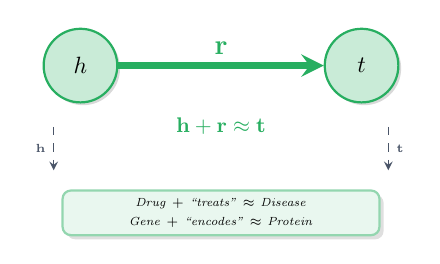
\begin{tikzpicture}[scale=0.85, transform shape]
        \node[technode, fill=transeGreen!25, draw=transeGreen,
              font=\normalsize\bfseries, minimum size=1.1cm] (h) at (0,0) {$h$};
        \node[technode, fill=transeGreen!25, draw=transeGreen,
              font=\normalsize\bfseries, minimum size=1.1cm] (t) at (4.2,0) {$t$};
        \draw[->,line width=2.5pt,>=stealth,color=transeGreen]
          (h) -- node[above,font=\large\bfseries,color=transeGreen]{$\mathbf{r}$} (t);
        \node[font=\small\bfseries, color=transeGreen] at (2.1,-0.9)
          {$\mathbf{h}+\mathbf{r}\approx\mathbf{t}$};
        \node[modernbox, fill=transeGreen!10, draw=transeGreen!50,
              text width=4.5cm, align=center, font=\tiny] at (2.1,-2.2)
          {\textit{Drug} + \textit{``treats''} $\approx$ \textit{Disease}\\[2pt]
           \textit{Gene} + \textit{``encodes''} $\approx$ \textit{Protein}};
        \draw[->,dashed,>=stealth,color=darkGray]
          ([shift={(-0.4cm,-0.35cm)}]h.south) --
          node[left,font=\tiny]{$\mathbf{h}$}
          ([shift={(-0.4cm,-1cm)}]h.south);
        \draw[->,dashed,>=stealth,color=darkGray]
          ([shift={(0.4cm,-0.35cm)}]t.south) --
          node[right,font=\tiny]{$\mathbf{t}$}
          ([shift={(0.4cm,-1cm)}]t.south);
      \end{tikzpicture}
    \end{column}
  \end{columns}
\end{frame}

\begin{frame}{TransE -- Come Funziona}
  \centering
  \vspace{0.1cm}
  % Ridotto lo scale a 0.75 per coerenza visiva e margini sicuri
  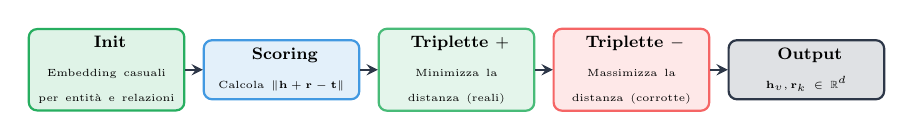
\begin{tikzpicture}[scale=0.75, transform shape, node distance=0.35cm]
    \node[rectangle,rounded corners=3pt,draw=transeGreen,thick,fill=transeGreen!15,
          text width=2.4cm,minimum height=1.0cm,text centered] (s1)
      {\footnotesize\textbf{\icoCogs\ Init}\\[2pt]{\tiny Embedding casuali per entit\`a e relazioni}};
    \node[rectangle,rounded corners=3pt,draw=accentBlue,thick,fill=accentBlue!15,
          text width=2.4cm,minimum height=1.0cm,text centered, right=0.3cm of s1] (s2)
      {\footnotesize\textbf{\icoNet\ Scoring}\\[2pt]{\tiny Calcola $\|\mathbf{h}+\mathbf{r}-\mathbf{t}\|$}};
    \node[rectangle,rounded corners=3pt,draw=successGreen,thick,fill=successGreen!15,
          text width=2.4cm,minimum height=1.0cm,text centered, right=0.3cm of s2] (s3)
      {\footnotesize\textbf{\icoThumb\ Triplette $+$}\\[2pt]{\tiny Minimizza la distanza (reali)}};
    \node[rectangle,rounded corners=3pt,draw=warningRed,thick,fill=warningRed!15,
          text width=2.4cm,minimum height=1.0cm,text centered, right=0.3cm of s3] (s4)
      {\footnotesize\textbf{\icoBan\ Triplette $-$}\\[2pt]{\tiny Massimizza la distanza (corrotte)}};
    \node[rectangle,rounded corners=3pt,draw=primaryDark,thick,fill=primaryDark!15,
          text width=2.4cm,minimum height=1.0cm,text centered, right=0.3cm of s4] (s5)
      {\footnotesize\textbf{\icoChart\ Output}\\[2pt]{\tiny $\mathbf{h}_v, \mathbf{r}_k \in \mathbb{R}^d$}};
    \draw[->,thick,>=stealth,color=primaryDark] (s1)--(s2);
    \draw[->,thick,>=stealth,color=primaryDark] (s2)--(s3);
    \draw[->,thick,>=stealth,color=primaryDark] (s3)--(s4);
    \draw[->,thick,>=stealth,color=primaryDark] (s4)--(s5);
  \end{tikzpicture}

  \vspace{0.4cm}
  \begin{columns}[T]
    \begin{column}{0.48\textwidth}
      \begin{block}{\icoCode\ Training con PyG}
        \footnotesize
        \texttt{from torch\_geometric.nn import TransE}\\
        \texttt{model = TransE(num\_nodes, num\_relations,}\\
        \texttt{\hspace{2.5em}hidden\_channels=50)}\\
        \texttt{loss = model.loss(head, rel, tail)}
      \end{block}
    \end{column}
    \begin{column}{0.48\textwidth}
      \begin{block}{\icoPlay\ Prediction con GDS}
        \footnotesize
        \texttt{gds.model.transe.create(G, "emb", ...)}\\
        \texttt{model.predict\_stream(}\\
        \texttt{\hspace{2em}source\_node\_filter=...,}\\
        \texttt{\hspace{2em}top\_k=3)}
      \end{block}
    \end{column}
  \end{columns}
\end{frame}

\begin{frame}{TransE -- PRO e CONTRO}
  \begin{columns}[T]
    \begin{column}{0.48\textwidth}
      \begin{block}{\icoThumb\ PRO}
        \footnotesize
        \begin{itemize}
          \setlength{\itemsep}{1pt}
          \setlength{\parskip}{0pt}
          \item[\pro] Apprende embedding per \textbf{tipo relazione}
          \item[\pro] Progettato per \textbf{Link Prediction} su KG
          \item[\pro] Ideale per grafi \textbf{eterogenei} (208 tipi)
          \item[\pro] Ottimi risultati su benchmark KG
        \end{itemize}
      \end{block}
    \end{column}
    \begin{column}{0.48\textwidth}
      \begin{alertblock}{\icoWarn\ CONTRO}
        \footnotesize
        \begin{itemize}
          \setlength{\itemsep}{1pt}
          \setlength{\parskip}{0pt}
          \item[\con] \textbf{Transductive}: non generalizza
          \item[\con] Difficolt\`a con relazioni \textbf{N:N}
          \item[\con] \textbf{Non usa feature} dei nodi
          \item[\con] Training \textbf{separato} da Neo4j (PyG)
        \end{itemize}
      \end{alertblock}
    \end{column}
  \end{columns}
  \vspace{-0.1cm}
  \begin{exampleblock}{\icoIdea\ Caso d'uso ideale}
    \footnotesize
    \textbf{Knowledge Graph} con relazioni eterogenee e task di \textbf{completamento KG}:
    drug-target interaction, gene-disease association.
    Dataset: FB15k-237, WN18RR, UMLS, PharMeBiNet.
  \end{exampleblock}
\end{frame}

\section{HashGNN}

\begin{frame}{HashGNN -- Cos'\`e}
  \begin{columns}[T]
    \begin{column}{0.50\textwidth}
      \begin{block}{\icoBrain\ Definizione}
        \small
        \textbf{Hashing-based Graph Neural Network}\\
        Algoritmo \textbf{unsupervised}: nonostante il nome,
        \textbf{non \`e un modello neurale}. Usa
        \textbf{Locality Sensitive Min-Hashing} (LSH) invece del
        gradiente. Ispirato al message passing dei GNN.
      \end{block}
      \vspace{0.2cm}
      \begin{exampleblock}{\icoIdea\ Idea Chiave}
        \small
        Le hash function sono \textbf{casuali e indipendenti} dai dati
        $\Rightarrow$ \textbf{nessun training necessario}.\\
        Velocissimo e scalabile anche senza GPU.
      \end{exampleblock}
    \end{column}
    \begin{column}{0.47\textwidth}
      \centering
      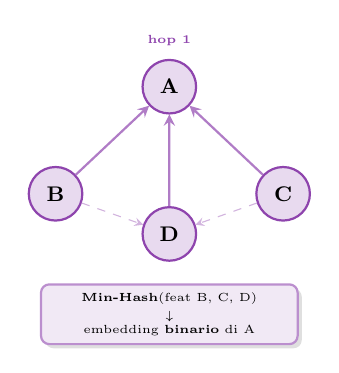
\begin{tikzpicture}[scale=0.85, transform shape,
        n/.style={circle, draw=hashgnnPurple, fill=hashgnnPurple!20,
                  thick, minimum size=0.8cm, font=\small\bfseries},
        arr/.style={->,thick,>=stealth,draw=hashgnnPurple!70}]
        \node[n] (a)  at (2,2.2)  {A};
        \node[n] (b)  at (0.3,0.6){B};
        \node[n] (c)  at (3.7,0.6){C};
        \node[n] (d)  at (2,0)    {D};
        \draw[arr] (b)--(a); \draw[arr] (c)--(a); \draw[arr] (d)--(a);
        \draw[->,dashed,>=stealth,draw=hashgnnPurple!40] (b)--(d);
        \draw[->,dashed,>=stealth,draw=hashgnnPurple!40] (c)--(d);
        \node[modernbox, fill=hashgnnPurple!12, draw=hashgnnPurple!60,
              font=\tiny, text width=3.6cm, align=center] at (2,-1.2)
          {\textbf{Min-Hash}(feat B, C, D)\\[2pt]$\downarrow$\\
           embedding \textbf{binario} di A};
        \node[font=\tiny, above=2pt of a, color=hashgnnPurple]
          {\textbf{hop 1}};
      \end{tikzpicture}
    \end{column}
  \end{columns}
\end{frame}

\begin{frame}{HashGNN -- Come Funziona}
  \centering
  \vspace{0.1cm}
  % Ridotto lo scale a 0.75 per coerenza visiva e margini sicuri
  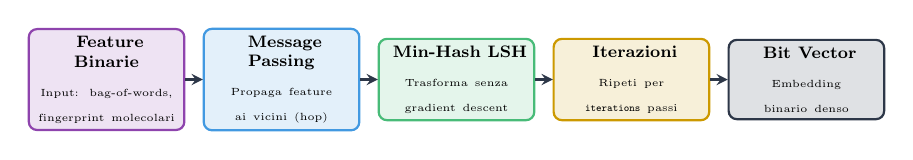
\begin{tikzpicture}[scale=0.75, transform shape, node distance=0.35cm]
    \node[rectangle,rounded corners=3pt,draw=hashgnnPurple,thick,fill=hashgnnPurple!15,
          text width=2.4cm,minimum height=1.0cm,text centered] (s1)
      {\footnotesize\textbf{\icoCode\ Feature Binarie}\\[2pt]{\tiny Input: bag-of-words, fingerprint molecolari}};
    \node[rectangle,rounded corners=3pt,draw=accentBlue,thick,fill=accentBlue!15,
          text width=2.4cm,minimum height=1.0cm,text centered, right=0.3cm of s1] (s2)
      {\footnotesize\textbf{\icoNet\ Message Passing}\\[2pt]{\tiny Propaga feature ai vicini (hop)}};
    \node[rectangle,rounded corners=3pt,draw=successGreen,thick,fill=successGreen!15,
          text width=2.4cm,minimum height=1.0cm,text centered, right=0.3cm of s2] (s3)
      {\footnotesize\textbf{\icoCogs\ Min-Hash LSH}\\[2pt]{\tiny Trasforma senza gradient descent}};
    \node[rectangle,rounded corners=3pt,draw=unigold,thick,fill=unigold!15,
          text width=2.4cm,minimum height=1.0cm,text centered, right=0.3cm of s3] (s4)
      {\footnotesize\textbf{\icoRocket\ Iterazioni}\\[2pt]{\tiny Ripeti per \texttt{iterations} passi}};
    \node[rectangle,rounded corners=3pt,draw=primaryDark,thick,fill=primaryDark!15,
          text width=2.4cm,minimum height=1.0cm,text centered, right=0.3cm of s4] (s5)
      {\footnotesize\textbf{\icoChart\ Bit Vector}\\[2pt]{\tiny Embedding binario denso}};
    \draw[->,thick,>=stealth,color=primaryDark] (s1)--(s2);
    \draw[->,thick,>=stealth,color=primaryDark] (s2)--(s3);
    \draw[->,thick,>=stealth,color=primaryDark] (s3)--(s4);
    \draw[->,thick,>=stealth,color=primaryDark] (s4)--(s5);
  \end{tikzpicture}

  \vspace{0.4cm}
  \begin{columns}[T]
    \begin{column}{0.48\textwidth}
      \begin{block}{\icoCode\ In Neo4j GDS}
        \footnotesize
        \texttt{gds.hashgnn.mutate(G, \{}\\
        \texttt{\hspace{1.5em}iterations: 4,}\\
        \texttt{\hspace{1.5em}heterogeneous: true,}\\
        \texttt{\hspace{1.5em}embeddingDensity: 512}\\
        \texttt{\})}
      \end{block}
    \end{column}
    \begin{column}{0.48\textwidth}
      \begin{block}{\icoNet\ Eterogeneità Nativa}
        \footnotesize
        Con \texttt{heterogeneous: true} HashGNN gestisce
        \textbf{automaticamente} nodi e relazioni di tipo diverso,
        senza proiezioni aggiuntive.
      \end{block}
    \end{column}
  \end{columns}
\end{frame}

\begin{frame}{HashGNN -- PRO e CONTRO}
  \begin{columns}[T]
    \begin{column}{0.48\textwidth}
      \begin{block}{\icoThumb\ PRO}
        \footnotesize
        \begin{itemize}
          \setlength{\itemsep}{1pt}
          \setlength{\parskip}{0pt}
          \item[\pro] \textbf{Nessun training}: hash random $\to$ istantaneo
          \item[\pro] Supporta grafi \textbf{eterogenei} nativamente
          \item[\pro] Ottimo per \textbf{Node Classification} multimodale
          \item[\pro] \textbf{Scalabilit\`a eccellente} in cluster GDS
          \item[\pro] Funziona senza \textbf{GPU}
        \end{itemize}
      \end{block}
    \end{column}
    \begin{column}{0.48\textwidth}
      \begin{alertblock}{\icoWarn\ CONTRO}
        \footnotesize
        \begin{itemize}
          \setlength{\itemsep}{1pt}
          \setlength{\parskip}{0pt}
          \item[\con] Richiede feature \textbf{binarie} o pre-processing
          \item[\con] \textbf{Non semantico}: ignora il \emph{tipo} delle rel.
          \item[\con] Embedding \textbf{binari}: meno espressivi
          \item[\con] Non adatto per \textbf{Link Prediction} semantica
        \end{itemize}
      \end{alertblock}
    \end{column}
  \end{columns}
  \vspace{-0.1cm}
  \begin{exampleblock}{\icoIdea\ Caso d'uso ideale}
    \footnotesize
    Grafi eterogenei con feature binarie disponibili: IMDB,
    grafi biomedici con \textbf{fingerprint molecolari}, ontologie. Ideale come
    \textbf{baseline rapida} prima di modelli pi\`u costosi.
  \end{exampleblock}
\end{frame}

\section{Comparazione Teorica}

\begin{frame}{Comparazione Visiva: i Tre Algoritmi}
  \centering
  \vspace{-0.2cm}
  % Ridotto a scale=0.75 per risolvere definitivamente l'Overfull \hbox
  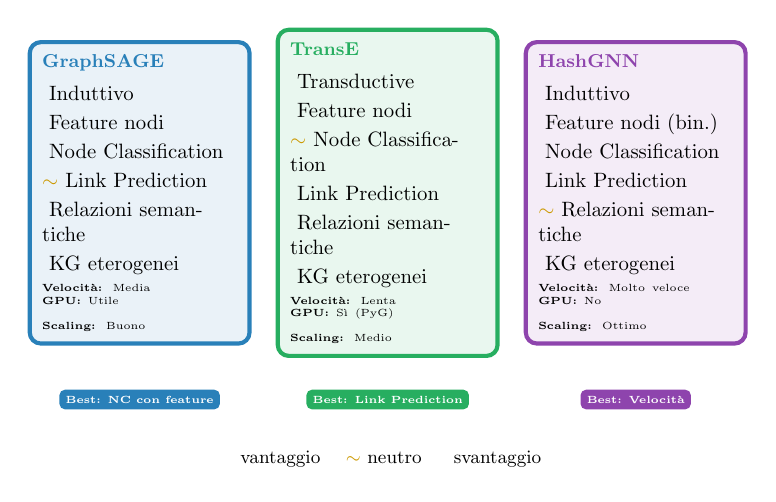
\begin{tikzpicture}[scale=0.75, transform shape]
    \node[rectangle,rounded corners=4pt,draw=graphsageBlue,line width=1.5pt,
          fill=graphsageBlue!10,minimum width=3.5cm,text width=3.3cm,
          align=left,inner sep=6pt] (gs) at (-4.2,0) {
      {\small\bfseries\color{graphsageBlue}GraphSAGE}\\[4pt]
      \pro\ Induttivo\\[2pt]
      \pro\ Feature nodi\\[2pt]
      \pro\ Node Classification\\[2pt]
      \neu\ Link Prediction\\[2pt]
      \con\ Relazioni semantiche\\[2pt]
      \con\ KG eterogenei\\[4pt]
      {\tiny\textbf{Velocit\`a:} Media\\
      \textbf{GPU:} Utile\\
      \textbf{Scaling:} Buono}
    };
    \node[rectangle,rounded corners=4pt,draw=transeGreen,line width=1.5pt,
          fill=transeGreen!10,minimum width=3.5cm,text width=3.3cm,
          align=left,inner sep=6pt] (tr) at (0,0) {
      {\small\bfseries\color{transeGreen}TransE}\\[4pt]
      \con\ Transductive\\[2pt]
      \con\ Feature nodi\\[2pt]
      \neu\ Node Classification\\[2pt]
      \pro\ Link Prediction\\[2pt]
      \pro\ Relazioni semantiche\\[2pt]
      \pro\ KG eterogenei\\[4pt]
      {\tiny\textbf{Velocit\`a:} Lenta\\
      \textbf{GPU:} S\`i (PyG)\\
      \textbf{Scaling:} Medio}
    };
    \node[rectangle,rounded corners=4pt,draw=hashgnnPurple,line width=1.5pt,
          fill=hashgnnPurple!10,minimum width=3.5cm,text width=3.3cm,
          align=left,inner sep=6pt] (hg) at (4.2,0) {
      {\small\bfseries\color{hashgnnPurple}HashGNN}\\[4pt]
      \pro\ Induttivo\\[2pt]
      \pro\ Feature nodi (bin.)\\[2pt]
      \pro\ Node Classification\\[2pt]
      \con\ Link Prediction\\[2pt]
      \neu\ Relazioni semantiche\\[2pt]
      \pro\ KG eterogenei\\[4pt]
      {\tiny\textbf{Velocit\`a:} Molto veloce\\
      \textbf{GPU:} No\\
      \textbf{Scaling:} Ottimo}
    };
    \node[fill=graphsageBlue, rounded corners=2pt, text=white,
          font=\tiny\bfseries, inner sep=3pt] at (-4.2,-3.5) {Best: NC con feature};
    \node[fill=transeGreen, rounded corners=2pt, text=white,
          font=\tiny\bfseries, inner sep=3pt] at (0,-3.5) {Best: Link Prediction};
    \node[fill=hashgnnPurple, rounded corners=2pt, text=white,
          font=\tiny\bfseries, inner sep=3pt] at (4.2,-3.5) {Best: Velocit\`a};
          
    \node[font=\small, align=center] at (0,-4.5) {\pro\ vantaggio \quad \neu\ neutro \quad \con\ svantaggio};
  \end{tikzpicture}
\end{frame}

\section{Node Classification vs Link Prediction}

\begin{frame}{Node Classification su PharMeBiNet}
  \begin{block}{\icoNet\ Definizione}
    \small
    Dato un nodo $v$, predire la sua \textbf{label/categoria}
    (es.\ tipo di farmaco, funzione proteica, categoria di malattia).
  \end{block}
  \vspace{0.1cm}
  \begin{columns}[T]
    \begin{column}{0.32\textwidth}
      \begin{block}{\color{graphsageBlue}\icoBrain\ GraphSAGE}
        \footnotesize
        \begin{itemize}
          \setlength{\itemsep}{1pt}
          \item[\pro] Embedding multi-hop
          \item[\pro] Inductive (nodi nuovi)
          \item[\pro] Feature continue
          \item[\neu] Richiede training
        \end{itemize}
        \vspace{2pt}
        {\scriptsize\textbf{Metrica}: F1-Macro}
      \end{block}
    \end{column}
    \begin{column}{0.32\textwidth}
      \begin{block}{\color{transeGreen}\icoBrain\ TransE}
        \footnotesize
        \begin{itemize}
          \setlength{\itemsep}{1pt}
          \item[\neu] Transductive
          \item[\con] No feature nodi
          \item[\neu] Classificatore extra
          \item[\neu] Utile se rel. discrim.
        \end{itemize}
        \vspace{2pt}
        {\scriptsize\textbf{Metrica}: Accuracy}
      \end{block}
    \end{column}
    \begin{column}{0.32\textwidth}
      \begin{block}{\color{hashgnnPurple}\icoBrain\ HashGNN}
        \footnotesize
        \begin{itemize}
          \setlength{\itemsep}{1pt}
          \item[\pro] Nativo per KG etero
          \item[\pro] Istantaneo, no GPU
          \item[\pro] Pipeline GDS
          \item[\con] Solo feature binarie
        \end{itemize}
        \vspace{2pt}
        {\scriptsize\textbf{Metrica}: F1-Macro}
      \end{block}
    \end{column}
  \end{columns}
\end{frame}

\begin{frame}{Link Prediction su PharMeBiNet}
  \begin{block}{\icoLink\ Definizione}
    \small
    Predire se esiste (o esister\`a) una \textbf{relazione specifica} tra due nodi
    (es.\ drug-target binding, gene-disease, drug-drug interaction).
  \end{block}
  \vspace{0.1cm}
  \begin{columns}[T]
    \begin{column}{0.32\textwidth}
      \begin{block}{\color{graphsageBlue}\icoLink\ GraphSAGE}
        \footnotesize
        \begin{itemize}
          \setlength{\itemsep}{1pt}
          \item[\neu] Op. ad hoc su emb.
          \item[\pro] Vicinato strutturale
          \item[\con] No tipo relazione
          \item[\neu] Solo rel.\ omogenee
        \end{itemize}
        \vspace{2pt}
        {\scriptsize\textbf{Metrica}: AUC-ROC}
      \end{block}
    \end{column}
    \begin{column}{0.32\textwidth}
      \begin{block}{\color{transeGreen}\icoLink\ TransE}
        \footnotesize
        \begin{itemize}
          \setlength{\itemsep}{1pt}
          \item[\pro] \textbf{Progettato} per LP KG
          \item[\pro] Score $\|\mathbf{h}{+}\mathbf{r}{-}\mathbf{t}\|$
          \item[\pro] 208 rel.\ semantiche
          \item[\con] Difficolt\`a N:N
        \end{itemize}
        \vspace{2pt}
        {\scriptsize\textbf{Metrica}: Hits@10, MRR}
      \end{block}
    \end{column}
    \begin{column}{0.32\textwidth}
      \begin{block}{\color{hashgnnPurple}\icoLink\ HashGNN}
        \footnotesize
        \begin{itemize}
          \setlength{\itemsep}{1pt}
          \item[\con] Non pensato per LP
          \item[\con] No semantica relazioni
          \item[\neu] Solo feature extractor
          \item[\con] Emb. binari limitanti
        \end{itemize}
        \vspace{2pt}
        {\scriptsize\textbf{Metrica}: AUC-ROC}
      \end{block}
    \end{column}
  \end{columns}
\end{frame}

\begin{frame}{Raccomandazioni per i Task}
  \begin{alertblock}{\icoRocket\ Raccomandazione per Node Classification}
    \small
    \textbf{HashGNN} come eccellente baseline rapida.
    \textbf{GraphSAGE} per raggiungere le performance massimali, specialmente se sono disponibili feature numeriche continue.
    \textbf{TransE} da usare solo indirettamente come estrattore di feature strutturali.
  \end{alertblock}
  \vspace{0.5cm}
  \begin{alertblock}{\icoRocket\ Raccomandazione per Link Prediction}
    \small
    \textbf{TransE} \`e il candidato naturale e indiscusso per la Link Prediction su un Knowledge Graph eterogeneo come PharMeBiNet. \`E l'unico a modellare esplicitamente la semantica e la direzione di tutti i 208 tipi di relazioni.
  \end{alertblock}
\end{frame}

\section{Predizione su PharMeBiNet}

\begin{frame}{Predizione Teorica su PharMeBiNet}
  \begin{alertblock}{\icoWarn\ Nota Metodologica}
    \small
    Predizioni basate su analisi \textbf{teorica}. I risultati sperimentali
    verificheranno o smentiranno queste ipotesi: \`e la parte centrale della tesi.
  \end{alertblock}
  \vspace{0.3cm}
  \begin{columns}[T]
    \begin{column}{0.48\textwidth}
      \centering
      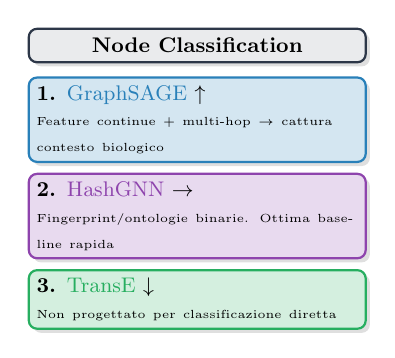
\begin{tikzpicture}[scale=0.85, transform shape]
        \node[modernbox, fill=primaryDark!10, text width=4.8cm,
              align=center, minimum height=0.5cm, font=\small\bfseries] (tt)
          {Node Classification};
        \node[modernbox, fill=graphsageBlue!20, draw=graphsageBlue,
              text width=4.8cm, align=left, font=\small,
              below=0.2cm of tt] (r1)
          {\textbf{1.} {\color{graphsageBlue}GraphSAGE} $\uparrow$\\
           {\tiny Feature continue + multi-hop $\to$ cattura contesto biologico}};
        \node[modernbox, fill=hashgnnPurple!20, draw=hashgnnPurple,
              text width=4.8cm, align=left, font=\small,
              below=0.15cm of r1] (r2)
          {\textbf{2.} {\color{hashgnnPurple}HashGNN} $\rightarrow$\\
           {\tiny Fingerprint/ontologie binarie. Ottima baseline rapida}};
        \node[modernbox, fill=transeGreen!20, draw=transeGreen,
              text width=4.8cm, align=left, font=\small,
              below=0.15cm of r2] (r3)
          {\textbf{3.} {\color{transeGreen}TransE} $\downarrow$\\
           {\tiny Non progettato per classificazione diretta}};
      \end{tikzpicture}
    \end{column}
    \begin{column}{0.48\textwidth}
      \centering
      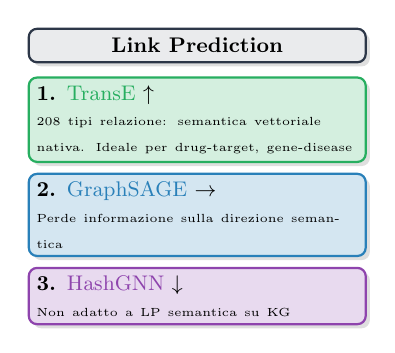
\begin{tikzpicture}[scale=0.85, transform shape]
        \node[modernbox, fill=primaryDark!10, text width=4.8cm,
              align=center, minimum height=0.5cm, font=\small\bfseries] (tt)
          {Link Prediction};
        \node[modernbox, fill=transeGreen!20, draw=transeGreen,
              text width=4.8cm, align=left, font=\small,
              below=0.2cm of tt] (r1)
          {\textbf{1.} {\color{transeGreen}TransE} $\uparrow$\\
           {\tiny 208 tipi relazione: semantica vettoriale nativa. Ideale per drug-target, gene-disease}};
        \node[modernbox, fill=graphsageBlue!20, draw=graphsageBlue,
              text width=4.8cm, align=left, font=\small,
              below=0.15cm of r1] (r2)
          {\textbf{2.} {\color{graphsageBlue}GraphSAGE} $\rightarrow$\\
           {\tiny Perde informazione sulla direzione semantica}};
        \node[modernbox, fill=hashgnnPurple!20, draw=hashgnnPurple,
              text width=4.8cm, align=left, font=\small,
              below=0.15cm of r2] (r3)
          {\textbf{3.} {\color{hashgnnPurple}HashGNN} $\downarrow$\\
           {\tiny Non adatto a LP semantica su KG}};
      \end{tikzpicture}
    \end{column}
  \end{columns}
\end{frame}

\section{Benchmark Prestazionale (1--2--4 Nodi)}

\begin{frame}{Setup del Cluster: Architettura}
  \centering
  \vspace{0.3cm}
  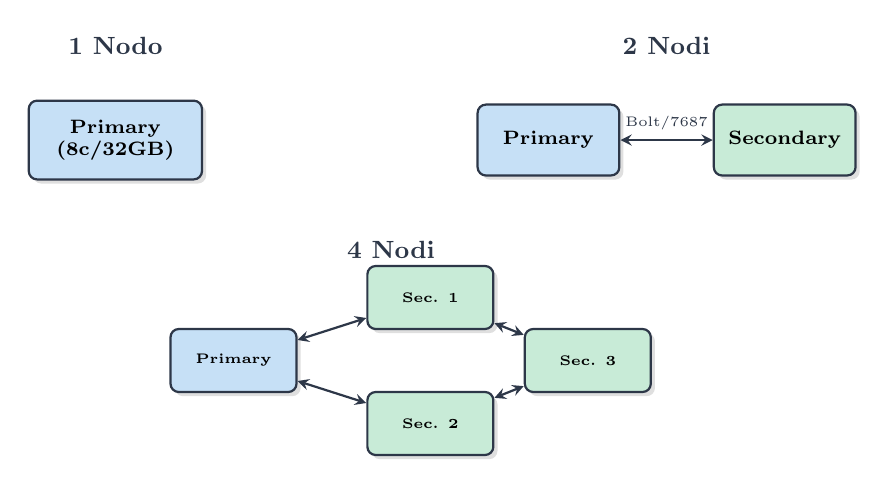
\begin{tikzpicture}[
    scale=1.0, transform shape,
    lbl/.style={font=\small\bfseries, color=primaryDark}
  ]
    \node[lbl] at (-3.5, 2.8) {1 Nodo};
    \node[modernbox, fill=accentBlue!30, minimum width=2.2cm,
          minimum height=1cm, align=center, font=\scriptsize\bfseries] (p1) at (-3.5, 1.6) {Primary\\(8c/32GB)};

    \node[lbl] at (3.5, 2.8) {2 Nodi};
    \node[modernbox, fill=accentBlue!30, minimum width=1.8cm,
          minimum height=0.9cm, align=center, font=\scriptsize\bfseries] (p2) at (2.0, 1.6) {Primary};
    \node[modernbox, fill=successGreen!30, minimum width=1.8cm,
          minimum height=0.9cm, align=center, font=\scriptsize\bfseries] (s2a) at (5.0, 1.6) {Secondary};
    \draw[<->,thick,>=stealth,color=primaryDark] (p2)--(s2a)
          node[midway,above,font=\tiny]{Bolt/7687};

    \node[lbl] at (0, 0.2) {4 Nodi};
    \node[modernbox, fill=accentBlue!30, minimum width=1.6cm, minimum height=0.8cm,
          align=center, font=\tiny\bfseries] (p4)  at (-2.0, -1.2)  {Primary};
    \node[modernbox, fill=successGreen!30, minimum width=1.6cm, minimum height=0.8cm,
          align=center, font=\tiny\bfseries] (s4a) at (0.5, -0.4) {Sec. 1};
    \node[modernbox, fill=successGreen!30, minimum width=1.6cm, minimum height=0.8cm,
          align=center, font=\tiny\bfseries] (s4b) at (0.5, -2.0) {Sec. 2};
    \node[modernbox, fill=successGreen!30, minimum width=1.6cm, minimum height=0.8cm,
          align=center, font=\tiny\bfseries] (s4c) at (2.5, -1.2) {Sec. 3};
    \draw[<->,thick,>=stealth,color=primaryDark] (p4)--(s4a);
    \draw[<->,thick,>=stealth,color=primaryDark] (p4)--(s4b);
    \draw[<->,thick,>=stealth,color=primaryDark] (s4a)--(s4c);
    \draw[<->,thick,>=stealth,color=primaryDark] (s4b)--(s4c);
  \end{tikzpicture}
\end{frame}

\begin{frame}{Setup del Cluster: Stack e Workflow}
  \begin{columns}[T]
    \begin{column}{0.48\textwidth}
      \begin{block}{\icoServer\ Azure Lab Services}
        \small
        \begin{itemize}
          \item[\icoCloud] Template: Win 10 Ent.\ LTSC 2021
          \item[\icoCogs] 8 core $\cdot$ 32 GB RAM per VM
          \item[\icoDocker] Docker Compose per Neo4j
          \item[\icoAnsible] Ansible: deploy automatico su tutte le VM
        \end{itemize}
      \end{block}
    \end{column}
    \begin{column}{0.48\textwidth}
      \begin{block}{\icoCogs\ Workflow di Deploy}
        \small
        \begin{enumerate}
          \item Template VM $\to$ Publish
          \item Ansible configura Primary + Secondary
          \item Apre porte firewall + WSL portproxy
          \item Avvia \texttt{docker compose up} su ogni nodo
          \item Verifica cluster da Primary
        \end{enumerate}
      \end{block}
    \end{column}
  \end{columns}
\end{frame}

\begin{frame}{Ipotesi Prestazionali sul Cluster}
  \begin{columns}[T]
    \begin{column}{0.32\textwidth}
      \begin{block}{\color{graphsageBlue}\icoBrain\ GraphSAGE}
        \footnotesize
        \begin{itemize}
          \setlength{\itemsep}{1pt}
          \item[\neu] GDS partial distrib.
          \item[\pro] Scaling \textbf{lineare} NC
          \item[\neu] RAM: alta (feat float)
          \item[\pro] Parallelismo nativo
          \item[\neu] Bottleneck: multi-hop
        \end{itemize}
        \vspace{4pt}
        {\scriptsize\textbf{Speedup}: buono (1$\to$4)}
      \end{block}
    \end{column}
    \begin{column}{0.32\textwidth}
      \begin{block}{\color{transeGreen}\icoBrain\ TransE}
        \footnotesize
        \begin{itemize}
          \setlength{\itemsep}{1pt}
          \item[\pro] Training distr. PyG
          \item[\neu] Scaling parziale
          \item[\neu] RAM: alta (KGE)
          \item[\neu] Query post-training
          \item[\con] Bottleneck: PyG
        \end{itemize}
        \vspace{4pt}
        {\scriptsize\textbf{Speedup}: medio (1$\to$4)}
      \end{block}
    \end{column}
    \begin{column}{0.32\textwidth}
      \begin{block}{\color{hashgnnPurple}\icoBrain\ HashGNN}
        \footnotesize
        \begin{itemize}
          \setlength{\itemsep}{1pt}
          \item[\pro] Istantaneo, no train
          \item[\pro] Scaling \textbf{ottimo}
          \item[\pro] RAM: bassa (bit vett.)
          \item[\pro] Parallelismo GDS
          \item[\neu] Bottleneck: hashing
        \end{itemize}
        \vspace{4pt}
        {\scriptsize\textbf{Speedup}: eccellente}
      \end{block}
    \end{column}
  \end{columns}
  \vspace{0.3cm}
  \begin{alertblock}{\icoRocket\ Predizione Globale}
    \small
    {\color{hashgnnPurple}\textbf{HashGNN}} sar\`a il pi\`u veloce in assoluto.
    {\color{transeGreen}\textbf{TransE}} beneficia meno della distribuzione (bottleneck PyG).
    {\color{graphsageBlue}\textbf{GraphSAGE}} mostrer\`a lo scaling pi\`u lineare su Node Classification.
  \end{alertblock}
\end{frame}

\begin{frame}{Metriche di Valutazione Pianificate}
  \begin{columns}[T]
    \begin{column}{0.48\textwidth}
      \begin{block}{\icoChart\ Metriche di Qualit\`a ML}
        \footnotesize
        \textbf{Node Classification:}
        \begin{itemize}
          \setlength{\itemsep}{1pt}
          \item[\icoStar] Accuracy, F1-Macro, F1-Weighted
          \item[\icoStar] Confusion Matrix per tipo nodo
        \end{itemize}
        \vspace{4pt}
        \textbf{Link Prediction:}
        \begin{itemize}
          \setlength{\itemsep}{1pt}
          \item[\icoStar] Mean Rank (MR), MRR
          \item[\icoStar] Hits@1, Hits@3, Hits@10
          \item[\icoStar] AUC-ROC
        \end{itemize}
      \end{block}
    \end{column}
    \begin{column}{0.48\textwidth}
      \begin{block}{\icoCogs\ Metriche Prestazionali}
        \footnotesize
        \begin{itemize}
          \setlength{\itemsep}{1pt}
          \item[\icoStar] \textbf{Training time} (ms) su 1, 2, 4 nodi
          \item[\icoStar] \textbf{Throughput} (embedding/sec)
          \item[\icoStar] \textbf{Memory footprint} GDS in-memory
          \item[\icoStar] \textbf{Speedup}: $S_n = T_1 / T_n$
          \item[\icoStar] \textbf{Efficienza}: $E_n = S_n / n$
        \end{itemize}
      \end{block}
      \vspace{-0.1cm}
      \begin{exampleblock}{\icoRoad\ Workflow Sperimentale}
        \footnotesize
        \begin{enumerate}
          \setlength{\itemsep}{1pt}
          \item EDA su PharMeBiNet
          \item Generazione embedding (3 algoritmi)
          \item Pipeline ML: NC + LP
          \item Benchmark 1/2/4 nodi $\to$ Analisi
        \end{enumerate}
      \end{exampleblock}
    \end{column}
  \end{columns}
\end{frame}

\begin{frame}{Sintesi e Prossimi Passi}
  \begin{columns}[T]
    \begin{column}{0.52\textwidth}
      \centering
      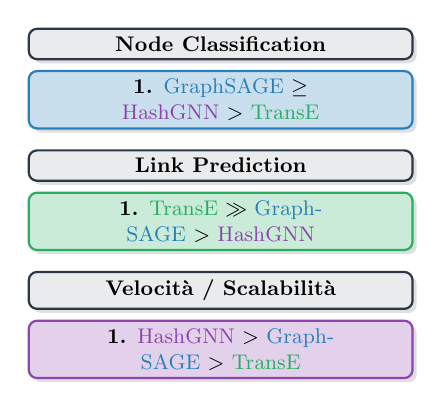
\begin{tikzpicture}[scale=0.85, transform shape]
        \node[modernbox, fill=primaryDark!10, text width=5.5cm,
              align=center, minimum height=0.45cm, font=\small\bfseries] (ncl)
          {Node Classification};
        \node[modernbox, fill=graphsageBlue!25, draw=graphsageBlue,
              text width=5.5cm, align=center, font=\small,
              below=0.15cm of ncl] (nc1)
          {\textbf{1.} {\color{graphsageBlue}GraphSAGE} $\geq$
           {\color{hashgnnPurple}HashGNN} $>$
           {\color{transeGreen}TransE}};
        \node[modernbox, fill=primaryDark!10, text width=5.5cm,
              align=center, minimum height=0.45cm, font=\small\bfseries,
              below=0.3cm of nc1] (lpl)
          {Link Prediction};
        \node[modernbox, fill=transeGreen!25, draw=transeGreen,
              text width=5.5cm, align=center, font=\small,
              below=0.15cm of lpl] (lp1)
          {\textbf{1.} {\color{transeGreen}TransE} $\gg$
           {\color{graphsageBlue}GraphSAGE} $>$
           {\color{hashgnnPurple}HashGNN}};
        \node[modernbox, fill=primaryDark!10, text width=5.5cm,
              align=center, minimum height=0.45cm, font=\small\bfseries,
              below=0.3cm of lp1] (spl)
          {Velocit\`a / Scalabilit\`a};
        \node[modernbox, fill=hashgnnPurple!25, draw=hashgnnPurple,
              text width=5.5cm, align=center, font=\small,
              below=0.15cm of spl] (sp1)
          {\textbf{1.} {\color{hashgnnPurple}HashGNN} $>$
           {\color{graphsageBlue}GraphSAGE} $>$
           {\color{transeGreen}TransE}};
      \end{tikzpicture}
    \end{column}
    \begin{column}{0.45\textwidth}
      \begin{alertblock}{\icoWarn\ Best-All-Round Previsto}
        \footnotesize
        \textbf{Non esiste un vincitore assoluto}: il migliore dipende
        dalla \textbf{task}. La tesi dimostrer\`a empiricamente i
        trade-off su PharMeBiNet.
      \end{alertblock}
      \vspace{0.2cm}
      \begin{block}{\icoRoad\ Prossimi Passi}
        \footnotesize
        \begin{enumerate}
          \item \icoServer\ Deploy Cluster su Azure
          \item \icoDB\ Caricare PharMeBiNet + EDA
          \item \icoCode\ Pipeline GDS/PyG (3 algo)
          \item \icoChart\ Benchmark 1 $\to$ 2 $\to$ 4 nodi
          \item \icoGrad\ Analisi risultati + stesura
        \end{enumerate}
      \end{block}
    \end{column}
  \end{columns}
\end{frame}
\end{document}